
\chapter{Shock Waves}\label{chap3}

WE\pageoriginale OBTAINED THE solution of the equation
$$
\rho_t+q_x=0
$$
on the assumptions
\begin{itemize}
\item [(1)] $\rho$ and $q$ are continuously differentiable.

\item [(2)] There exists a functional relation between $q$ and $\rho$; that is $q=Q(\rho)$. 
\end{itemize}

In our discussions we found the phenomena of breaking in some cases. At the time of breaking we have to reconsider our assumptions. We will approach this in two directions.
\begin{itemize}
\item [(i)] We still assume a functional relation between $q$ and $\rho$ i.e. $q = Q(\rho)$, but allow jump discontinuities for $\rho$ and $q$.

\item [(ii)] We assume $\rho$ and $q$ are continuously differentiable and $q$ is a function of $\rho$ and $\rho_x$. For simplicity we take this in the form
$$
q=Q(\rho)-\nu\rho_x 
$$
where $\nu >0$. 
\end{itemize}

\section{Discontinuous shocks}\label{chap2:sec3.1}

We now work with the assumption (i). Our conservation equation in the integrated form:
$$
\frac{d}{dt}\int\limits_{x_2}^{x_1}\rho\,dx+q_1-q_2=0
$$
still\pageoriginale holds even if $\rho$ and $q$ have jump discontinuities.

We now assume that the function $\rho(x,t)$ has a jump discontinuity at $x=s(t)$, where $s$ is a continuously differentiable function of $t$.

At time $t$, let $x_1>s(t)>x_2$ and $U(t)=s(t)=\frac{ds}{dt}$. The conservation equation can now be written as 
$$
\frac{d}{dt}\left\{\int\limits_{x_2}^{s(t)-}\rho\,dx+\int\limits_{s(t)+}^{x_1}\rho e\,dx\right\}+q_1-q_2=0
$$
This implies
\begin{gather*}
\int\limits_{x_2}^{s(t)-}\rho_t\,dx+s(t)\rho\,(s(t)-,t)+\int\limits_{s(t)+}^{x_1} \rho_t\,dx\\
-s(t)\rho \,(s(t)+,t)+q(x_1,t)-q(x_2,t)=0
\end{gather*}
Taking the limits $x_2\to s(t)-$ and $x_1\to s(t)+$ we obtain 
$$
-s(t)(\rho(s(t)+,t)-\rho(s(t)-,t))+(q(s(t)+,t)-q(s(t)-,t))=0
$$
We symbolically write this as
\begin{equation}
-U[\rho]+[q]=0\tag{3.1}\label{chap3:eq3.1}
\end{equation}
where $[.]$ denotes the jump.

\noindent Equation \eqref{chap3:eq3.1} is called the `shock condition'.

The basic problem can now be written as 
\begin{equation}
\begin{aligned}
&\rho_t+q_x=0,\quad\text{at points of continuity}\\
& -U[\rho]+[q]=0,\quad\text{at discontinuity points}
\end{aligned}\tag{3.2}\label{chap3:eq3.2}
\end{equation}

There is a nice correspondence between the differential equation and the shock condition.
$$
\frac{\partial}{\partial t}\leftrightarrow -U[.],\frac{\partial}{\partial x} \leftrightarrow [.].
$$\pageoriginale 

The shock condition can also be written as 
\begin{equation}
U=\frac{q_2-q_1}{\rho_2-\rho_1}=\frac{Q(\rho_2)-Q(\rho_1)}{\rho_2-\rho_1} \tag{3.3}\label{chap3:eq3.3}
\end{equation}
where the suffixes 1 and 2 stand for the arguments $(s(t)+,t)$ and $(s(t)-,t)$ respectively.

It is important to note that the {\bf direct} association of a jump condition with a differential equation in conservation form is not unique. For example, consider
\begin{equation}
\rho_t+\rho\rho_x=0\tag{3.4}\label{chap3:eq3.4}
\end{equation}
This can be written as $\rho_t+(\frac{1}{2}\rho^2)_x=0$, and the corresponding jump condition is 
\begin{equation}
-U[\rho]+\left[\frac{1}{2}\rho^2\right]=0\tag{3.5}\label{chap3:eq3.5}
\end{equation}
However, equation \eqref{chap3:eq3.4} can also be written as 
$$
\left(\frac{1}{2}\rho^2\right)_t +\left(\frac{1}{3}\rho^3\right)_x=0;
$$
the associated shock condition would be 
\begin{equation}
-U\left[\frac{1}{2}\rho^2\right]+\left[\frac{1}{3}\rho^3\right]=0 \tag{3.6}\label{chap3:eq3.6}
\end{equation}
Obviously \eqref{chap3:eq3.5} and \eqref{chap3:eq3.6} are different.

We have to choose the appropriate jump condition only from the physical considerations of the problem and the original {\bf integrated} form of the conservation law.

We now give the simplest example in which a shock occurs.

\begin{example*}
The\pageoriginale simplest case in which breaking occurs will be 
\begin{align*}
&\rho_t +c(\rho)\rho_x =0\quad\text{in}\quad t>0, \, -\infty < x < \infty,\\
&t=0:\rho=
\begin{cases}
\rho_2\quad\text{if}\quad x<0\\
\rho_1\quad\text{if}\quad x>0, \, \left(\rho_2>\rho_1\right)
\end{cases}
\end{align*}
with $c'(\rho)>0$
\begin{figure}[H]
\centering
\includegraphics{figures/fig61-3.1.eps}
\caption{}
\label{chap1:fig3.1}
\end{figure}

In this case breaking will occur immediately. The proposed discontinuous solution is just a shock moving with velocity
$$
U=\frac{Q\left(\rho_2\right)-Q\left(\rho_1\right)}{\rho_2 - \rho_1}
$$
an separating uniform regions $\rho=\rho_1$ and $\rho=\rho_2$ on the two sides.
\end{example*}

\section{Equal area rule}\label{chap3:sec3.2}
 
The general question of fitting in a discontinuous shock to replace a multivalued region can be answered elegantly by the following argument. The integrated form of the conservation equation, \ie,
$$
\frac{d}{dt}\int\limits_{x_2}^{x_1}\rho \,dx +q_1 -q_2 =0,
$$
holds for both the multivalued solution and the discontinuous solution.\pageoriginale If we take the case of a single hump disturbance as shown in the figure 3.2(a), with $\rho=\rho_0$ on both sides of the disturbance, and if we take $x_1, x_2$ far away from the disturbance with $q_1=q_2=Q(\rho_0)$, then
$$
\int\limits_{x_2}^{x_1}\rho\,dx =\quad\text{constant in time}
$$
This is so for both the multivalued solution in figure 3.2(b) and the discontinuous solution in figure 3.2(c). Hence the position of the shock must be chosen to give equal areas $A=B$ for the two lobes as shown in figure 3.2(d).

The analytic implementation of this construction is described in \cite{key1}
\begin{figure}[H]
\centering
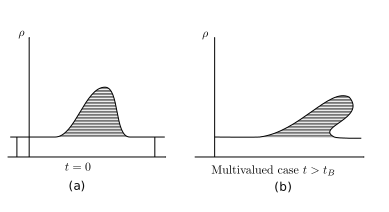
\includegraphics{figures/fig61-3.2ab.eps}
\medskip
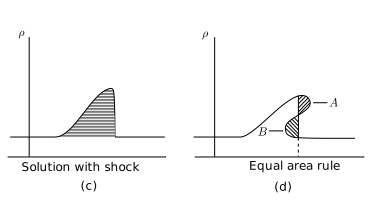
\includegraphics{figures/fig61-3.2cd.eps}
\caption{}
\label{chap1:fig3.2}
\end{figure}

\section{Asymptotic behavior}\pageoriginale \label{chap3:sec3.3}

We are interested in finding out what happens to the solution as $t\to \infty$, and this can be obtained directly without going through the previous construction in detail. We first study a special $Q(\rho)$ which simplifies the results.

The equation is,
\begin{equation}
\rho_t + q_x=0\tag{3.7}\label{chap3:eq3.7}
\end{equation}
with the shock condition
\begin{equation}
-U[\rho]+[q]=0\tag{3.8}\label{chap3:eq3.8}
\end{equation}

If $q=Q(\rho)$ and $c(\rho)=Q'(\rho)$ then, as noted already, \eqref{chap3:eq3.7} can be written as 
$$
C_t +CC_x=0,\quad\text{or}\quad C_t +\left(\frac{1}{2}C^2\right)_x=0
$$
where $C(x,t)=c(\rho(x,t))$. From the second form of the equation for $C$, we may be tempted to write the shock condition \eqref{chap3:eq3.8} as $-U[C]+[\frac{1}{2}C^2]=0$. But this is not always true, \ie conservation of $\rho$ does not imply the conservation of $C$. However, when $Q$ is quadratic, say,
$$
Q(\rho)=\alpha\rho^2 +\beta\rho +\gamma
$$
then conservation of $\rho$ implies the conservation of $C$, since $C$ is linear in $\rho$.

This can be easily checked as follows: We have
$$
c(\rho=Q'(\rho)=2\alpha\rho +\beta;
$$
by equation \eqref{chap3:eq3.8},
\begin{equation}
-U[\rho]+\left[\alpha\rho^2 +\beta\rho +\gamma\right]=0 \tag{3.9}\label{chap3:eq3.9}
\end{equation}\pageoriginale

Now,
\begin{multline*}
-U[C]+\frac{1}{2}\left[C^2\right]=-U[2\alpha\rho +\beta]+\left[2\alpha^2\rho^2+2\alpha \beta\rho+\frac{1}{2}\beta^2\right]\\
=2\alpha\left\{-U[\rho]+\left[\alpha\rho^2+\beta\rho +\gamma\right]\right\},
\end{multline*}
and this is seen to be zero by \eqref{chap3:eq3.9}. (Here we have used $[\beta]= [\frac{1}{2}\beta^2]=[\gamma]=0$ since $\beta$ and $\gamma$ are constants).

In this case we can work with $C$ alone and the shock condition is 
$$
U=\frac{c_1+c_2}{2}
$$

The initial value problem is
\begin{equation}
\left.
\begin{aligned}
&C_t+CC_x=0,\, t>0,\, -\infty < x < \infty\\
&C=F(x),\,t=0:\, -\infty < x < \infty.
\end{aligned}
\right\}\tag{3.10}\label{chap3:eq3.10}
\end{equation}

We will now consider the asymptotic behavior of a single hump, \ie 
\begin{equation*}F(\xi)=
\begin{cases}
c_0\quad\text{in}\quad x\leq a\\
g(x)\quad\text{in}\quad [a,L]\\
c_0\quad\text{in}\quad x\geq L
\end{cases}
\end{equation*}
where $g$ is continuous in $ [a,L]$ with $g(a)=g(L)=c_0$, as shown in figure 3.2(a).

In this case breaking will occur at the front and we fit a shock to remove multivaluedness. As time increases, much of the initial detail is lost. As this process is continued, it is plausible to reason that the remaining disturbance becomes linear in\pageoriginale $x$. In any event, there is such a simple solution with $C=x/t$. We propose, therefore, that the solution is 
\begin{equation}
C=
\begin{cases}
c_0, & x\leq c_0t\\
\frac{x}{t}, &c_0t\leq x\leq s(t),\\
c_0,&s(t)<x,
\end{cases}\tag{3.11}\label{chap3:eq3.11}
\end{equation}
where $x=s(t)$ is the position of the shock still to be determined.

The shock condition is $U=\frac{c_1+c_2}{2}$; therefore, since $c_1=c_0,c_2=s(t)/t$, we have 
\begin{equation}
\frac{ds}{dt}=\frac{1}{2}\left\{c_0+\frac{s}{t}\right\} \tag{3.12}\label{chap3:eq3.12} 
\end{equation}

The solution of this is easily found to be 
$$
S=c_0t+bt^{1/2},
$$
where $b$ is a constant. So we have a triangular wave for $C$ as shown in figure 3.3. The area of the triangle is $\frac{1}{2}b^2$ and this must remain equal to the area $A$ under the initial hump. Hence $b=(2A)^{1/2}$. Only the area of the initial wave appears in this final asymptotic solution; all other details are lost. It shold be remarked that this behavior is completely different from linear theory.
\begin{figure}[H]
\centering
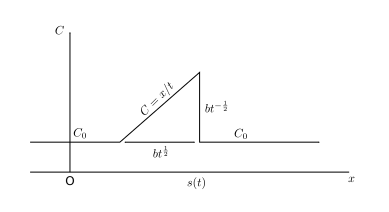
\includegraphics{figures/fig61-3.3.eps}
\caption{}
\label{chap1:fig3.3}
\end{figure}


\bigskip

{\bf \large Problems.}\pageoriginale
\begin{enumerate}
\item Solve
\begin{align*}
&\left(\frac{\partial}{\partial t}+u\frac{\partial}{\partial x}\right)\; \left(\frac{\partial}{\partial t}+u\frac{\partial}{\partial x}\right)u+u=0, \,t>0, \, -\infty < x < \infty,\\
& t=0:
\begin{cases}
u=0,\\
u_t=a\sin \,kx, \; -\infty < x < \infty
\end{cases}
\end{align*}
using the method of characteristics. Find also the time of first occurence of singularities.
\item Solve 
\begin{gather*}
\rho_t+\rho\rho_x=0, \, t>0, \, -\infty < x < \infty,\\
t=0:\rho=
\begin{cases}
0\quad\text{in}\quad x\leq 0\\
x\quad\text{in}\quad 0\leq x \leq\frac{1}{2}\\
1-x\quad\text{in}\quad \frac{1}{2}\leq x\leq 1\\
0\quad\text{in}\quad x\geqq 1
\end{cases}
\end{gather*}
Find the first time of breaking and the point at which it breaks. Fit a shock to this and find the shock velocity.
\item solve 
\begin{gather*}
C_t+CC_x=0, \, t>0, \, -\infty < x < \infty,\\
t=0:c=
\begin{cases}
c_0\quad\text{in}\quad x\leqq 0\\
f(x)\quad\text{in}\quad [0,1]\\
c_0\quad\text{in} \quad x\geq 1
\end{cases}
\end{gather*}
where $f(x)$ is continuous in $[0,1]$ with $f(0)=f(1)=c_0$, $f$ decreases in $[0,\frac{1}{2}]$ and increases in $[\frac{1}{2},1]$. Show that breaking occurs. Describe the asymptotic behavior of the solution including\pageoriginale the shock.
\item The equation is the same as in the problem 3. Now the initial distribution is 
\begin{equation*}
t=0:f=
\begin{cases}
C_0\quad\text{in}\quad x\leqq -1\\
g(x)\quad\text{in}\quad [-1,1]\\
C_0\quad\text{in}\quad x\geqq 1
\end{cases}
\end{equation*}
where $g$ is a continuous function with $g(0)=g(-1)=g(1)=C_0, g$ is decreasing in $[-1,\frac{1}{2}]$ and increasing in $[-\frac{1}{2},\frac{1}{2}]$ and again decreasing in $[\frac{1}{2},1]$. Fit shocks wherever necessary and find the asymptotic behavior of the solution. The asymptotic form is called an N-wave.

\item Solve
\begin{align*}
C_t +CC_x&=0, \,t>0, \, -\infty < x < \infty,\\
t=0: C&=F(\xi)=C_0+a\sin\frac{2\pi\xi}{\lambda}
\end{align*}
Use the fact that $C=\frac{x}{t}$ is a solution of the equation to describe the asymptotic behavior of the solution. Deduce that the asymptotic solution is independent of `$a$' and that the shock decays like $t^{-1}$ rather than $t^{1/2}$. Note that the area under the initial curve in the left interval $[0,\lambda/2]$ is not preserved.

\item Assuming that shocks are only required when breaking occurs show that the shock velocity lies between $C_1$ and $C_2$. 
\end{enumerate}

\section{Shock structure}\label{chap3:sec3.4}

In the first approach to resolve breaking we have assumed a\pageoriginale functional relation in $\rho$ and $q$ with appropriate shock conditions. Now we consider the second approach, namely that $q$ and $\rho$ are continuously differentiable but that $q$ is a function of $\rho$ and $\rho_x$. For simplicity we take 
\begin{equation}
q=Q(\rho)-\nu\rho_x\tag{3.13}\label{chap3:eq3.13}
\end{equation}
where $\nu > 0$. (Here the sign of $\nu$ is important). When $\rho_x$ is small, $q=Q(\rho)$ is a good approximation; but near breaking where $\rho_x$ is large, \eqref{chap3:eq3.13} gives a better approximation. A motivation for \eqref{chap3:eq3.13} can be seen from traffic flow. In traffic flow, the density $\rho$ is the number of cars per unit length. When the density is increasing ahead, $\rho_x >0$, one expects the drivers to adjust the speed a little below equilibrium $q=Q(\rho)$, and when $\rho_x<0$ perhaps a little above. This is represented by the extra term $\nu\rho_x$ in \eqref{chap3:eq3.13}. The other examples in chapter have similar correction terms in an improved description.

The conservation equation is 
$$
\frac{d}{dt}\int\limits_{x_2}^{x_1}\rho\,dx +q_1 -q_2 =0
$$
and for differentiable $\rho,q$ we have the differential equation 
\begin{equation}
\rho_t+q_x=0\tag{3.14}\label{chap3:eq3.14}
\end{equation}
as before. Using \eqref{chap3:eq3.13}, \eqref{chap3:eq3.14} becomes 
\begin{equation}
\rho_t+c(\rho)\rho_x=\nu\rho_{xx}\tag{3.15}\label{chap3:eq3.15}
\end{equation}
where\pageoriginale $c(\rho)=Q'(\rho)$. Before considering the solution of \eqref{chap3:eq3.15} in detail, we note the general qualitative effects of the terms $c(\rho)\rho_x$ and $\nu\rho_{xx}$. To see this we take the initial function to be a step function. 
\begin{equation}
t=0:\rho=
\begin{cases}
\rho_2\quad\text{if}\quad x<0\\
\rho_1\quad\text{if}\quad x>0
\end{cases}\tag{3.16}\label{chap3:eq3.16}
\end{equation}
with $\rho_2>\rho_1$. Omitting the term $c(\rho).\rho_x$, the equation \eqref{chap3:eq3.15} becomes the heat equation,
\begin{equation}
\rho_t=\nu\rho_{xx}\tag{3.17}\label{chap3:eq3.17}
\end{equation}

The solution to \eqref{chap3:eq3.17} with the initial conditions \eqref{chap3:eq3.16} is 
\begin{equation}
\rho=\rho_2-\frac{\rho_2-\rho_1}{\sqrt{\pi}}\int\limits_{-\infty}^{\frac{x}{\sqrt{4\nu t}}} e^{-\zeta^2}\,d\zeta\tag{3.18}\label{chap3:eq3.18}
\end{equation}

This shows that the effect of the term $\nu\rho_{xx}$ is to smooth out the initial distribution like $(\nu t)^{-1/2}$. 

Neglecting the term $\nu\rho_{xx}$ in \eqref{chap3:eq3.15} we have the immediate breaking discussed earlier.

Thus our equation \eqref{chap3:eq3.15} will have both the effects, namely stretching and steepening, and it seems reasonable that there will be solutions having the balance between the two. We will now look for simple solutions to test the idea. Let us assume that 
\begin{equation}
\rho =\rho(X), X=x-Ut\tag{3.19}\label{chap3:eq3.19}
\end{equation}
is a solution of \eqref{chap3:eq3.15}, where $U$ is a constant. We also assume that
\begin{equation}
\left.
\begin{aligned}
&\rho\to\rho_1\quad\text{as}\quad x\to \infty\\
&\rho\to\rho_2\quad\text{as}\quad x\to -\infty\\
\text{and}\quad &\rho_x\to 0\quad\text{as}\quad x\to \pm\infty
\end{aligned}\tag{3.20}\label{chap3:eq3.20}
\right\}
\end{equation}\pageoriginale

Now \eqref{chap3:eq3.15} becomes 
\begin{equation}
c(\rho)\rho_X-U\rho_X=\nu\rho_{XX}\tag{3.21}\label{chap3:eq3.21}
\end{equation}

Using $c(\rho)=Q'(\rho)$ and integrating \eqref{chap3:eq3.21} with reference to $X$ we obtain
\begin{equation}
Q(\rho)-U\rho +A=\nu_{\rho_{X}},\tag{3.22}\label{chap3:eq3.22}
\end{equation}
where $A$ is the constant of integration. Equations \eqref{chap3:eq3.22} and \eqref{chap3:eq3.20} imply
$$
U=\frac{Q(\rho_2)-Q(\rho_1)}{\rho_2-\rho_1}
$$
which is exactly the same as the shock velocity in the discontinuity theory. Equation \eqref{chap3:eq3.22} can be written as 
$$
\frac{1}{\nu}=\frac{1}{Q(\rho)-U\rho+A}\cdotp \frac{d\rho}{dX}\cdotp
$$

Integrating this with reference to $X$ we get 
\begin{equation}
\frac{X}{\nu}=\int\frac{d\rho}{Q(\rho)-U\rho+A}\tag{3.23}\label{chap3:eq3.23}
\end{equation}

Since $\rho_1,\rho_2$ are zeroes of $Q(\rho)-U\rho+A$ the integrals taken over the neighbourhoods of $\rho_1,\rho_2$ diverge; so $X\to \pm\infty$ as $\rho\to\rho_1$ or $\rho_2$. This is consistent with our assumptions \eqref{chap3:eq3.20}. 

If $c'(\rho)>0$ then $Q(\rho)\leqq U\rho - A$ in $[\rho_1,\rho_2]$ and then by \eqref{chap3:eq3.22} $\rho_X\leqq 0$. Hence $\rho$ is decreasing and the solution can be schematically\pageoriginale represented as in figure 3.4.
\begin{figure}[H]
\centering
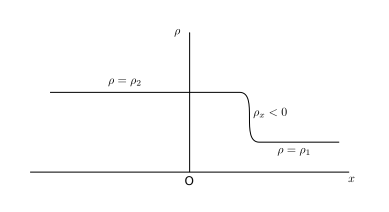
\includegraphics{figures/fig61-3.4.eps}
\caption{}
\label{chap1:fig3.4}
\end{figure}


An explicit solution for \eqref{chap3:eq3.15} and \eqref{chap3:eq3.16} can be obtained when $Q$ is the quadratic 
$$
Q=\alpha\rho^2+\beta\rho +\gamma
$$

Then
$$
Q(\rho)-U\rho +A= -\alpha\left(\rho -\rho_1\right),\; \left(\rho_2-\rho\right),
$$
and by \eqref{chap3:eq3.23}
\begin{align*}
\frac{X}{\nu} &= -\int \frac{d\rho}{\alpha(\rho_2-\rho)\;(\rho-\rho_1)}\\
&= \frac{1}{\alpha\left(\rho_2-\rho_1\right)}\log \left(\frac{\rho_2-\rho}{\rho-\rho_1}\right).
\end{align*}

Hence we obtain a solution 
\begin{equation*}
\rho=\rho_1+\left(\rho_2-\rho_1\right)\frac{\exp\left(-\left(\rho_2-\rho_1\right) \alpha X/\nu\right)}{1+\exp\left(-\left(\rho_2-\rho_1\right)\alpha X/\nu\right)} \tag{3.24}\label{chap3:eq3.24}
\end{equation*}

When $\nu$ is small, the transition region between $\rho_1$ to $\rho_2$ is very thin. This can be made more precise as follow $s$.

Consider the tangent through the point of inflexion of the curve\pageoriginale $\rho$ in the $\rho-X$ Plane. Let it cut the lines $\rho=\rho_1$, and $\rho=\rho_2$ at the points $(X_1,\rho_1)$ and $(X_2,\rho_2)$ respectively. The difference between $X_1$ and $X_2$ is called the `shock thickness'. 
\begin{figure}[H]
\centering
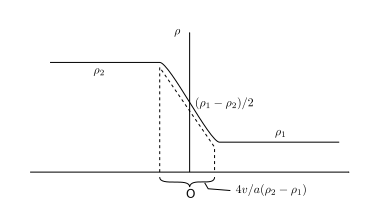
\includegraphics{figures/fig61-3.5.eps}
\caption{}
\label{chap1:fig3.5}
\end{figure}

In the particular case \eqref{chap3:eq3.24} we find the shock
thickness to be $4\nu/\alpha\break(\rho_2-\rho_1)$. From this we conclude
that the thickness tends to zero as $\nu$ tends to zero for fixed
$\rho_1,\rho_2$. However, notice that for fixed $\nu$ the thickness
eventually increases as $\rho_2-\rho_1\to 0$. 

In the improved theory this smooth, but rapid, transition layer replaces the discontinuous shock of the earlier theory. Similarly, we expect the discontinuities in more general solutions to be replaced by thin transition layers in the improved theory. This can be shown in full detail for the case of quadratic $Q(\rho)$ as explained in the next section.

\section{Burger's equation}\label{chap3:sec3.5}

Multiplying both sides of the equation \eqref{chap3:eq3.15} by $c'(\rho)$ and manipulating we obtain 
\begin{equation}
C_t+CC_x=\nu C_{xx}+\nu c''(\rho)\rho_x^2\tag{3.25}\label{chap3:eq3.25}
\end{equation}

In\pageoriginale the special case when $Q(\rho)$ is again the quadratic $\alpha\rho^2 +\beta\rho+\gamma$ we have $c''(\rho)=0$. Hence \eqref{chap3:eq3.25} becomes
\begin{equation*}
C_t+CC_x=\nu C_{xx} \tag{3.26}\label{chap3:eq3.26}
\end{equation*}

Equation \eqref{chap3:eq3.26} is called Burgers' equation. This equation is originally due to Bateman (1935) but Burgers gave special solutions to it in 1940 and emphasized its importance. In 1950--51 Cole and Holf worked independently on this and solved it explicitly. They introduced a non-linear transformation which converted \eqref{chap3:eq3.26} into the linear heat equation. We now give a brief account of this transformation.

First, if we introduce the variable
\begin{equation}
C=\Psi_{x},\tag{3.27}\label{chap3:eq3.27}
\end{equation}
equation \eqref{chap3:eq3.26} becomes 
$$
\Psi_{xt}+\Psi_x.\Psi_{xx}=\nu\Psi_{xxx}.
$$

Integrating this with reference to $x$ we obtain
\begin{equation}
\Psi_t+\frac{1}{2}\Psi_x^2=\nu\Psi_{xx}.\tag{3.28}\label{chap3:eq3.28}
\end{equation}

The transformation
\begin{equation}
\Psi =-2\nu\log \phi\tag{3.29}\label{chap3:eq3.29}
\end{equation}
converts the equation \eqref{chap3:eq3.28} into the linear heat equation 
\begin{equation}
\phi_t=\nu\phi_{xx}\tag{3.30}\label{chap3:eq3.30}
\end{equation}

The initial condition
$$
t=0:\; C=F(x)
$$
for \eqref{chap3:eq3.26} becomes
\begin{equation}
t=0:\phi =\phi(\eta)=\exp\left\{-\frac{1}{2\nu}\int\limits_0F(x)\,dx \right\}\tag{3.31}\label{chap3:eq3.31}
\end{equation}\pageoriginale
Then the solution of \eqref{chap3:eq3.30} with the initial condition \eqref{chap3:eq3.31} is 
\begin{align*}
\phi(x,t) &= \frac{1}{\sqrt{4\pi\nu t}}\int\limits_{-\infty}^{\infty}\Phi (\eta)\exp\left\{-\frac{(x-\eta)^2}{4\nu t}\right\}\,d\eta\\
\intertext{and therefore,}
C(x,t) &= \frac{\int\limits_{-\infty}^\infty \frac{x-\eta}{t}.\Phi(\eta)\exp \left\{-\frac{(x-\eta)^2}{4\nu t}\right\}\,d\eta} {\int\limits_{-\infty}^\infty \Phi(\eta)\exp\left\{-\frac{(x-\eta)^2}{4 t}\right\}\,d\eta}
\end{align*}

The counterparts of the various solutions discussed in the discontinuity theory can be studied in this improved theory. Except for extremely weak shocks in certain cases, the only significant change (for small $\nu$) is the smoothing of the shocks into thin transition layers. A full account is given in \cite{key1}.

\section{Chemical exchange processes; Thomas's equation}\label{chap3:sec3.6}

The situation is similar in chemical exchange processes. The conservation equation is 
\begin{equation}
\frac{\partial}{\partial t}\left(\rho_f+\rho_s\right)+\frac{\partial}{\partial x} \left(V\rho_f\right)=0\tag{3.32}\label{chap3:eq3.32}
\end{equation}
where $\rho_f,\rho_s$ are as before (see section \ref{chap2:sec2.3}. We took 
\begin{equation}
\rho_s=R\left(\rho_f\right)\tag{3.33}\label{chap3:eq3.33}
\end{equation}
to be an approximation and obtained the one dimensional non-linear wave equation. In many cases a more detailed description for the second relation between $\rho_f$ and $\rho_s$ is 
\begin{equation}
\frac{\partial\rho_s}{\partial t}=K_1\left(A-\rho_s\right)\rho_f-K_2\rho_s\left(B-\rho_f\right) \tag{3.34}\label{chap3:eq3.34}
\end{equation}\pageoriginale
where $K_1, K_2, A,B$ are constants. $A,B$ represent the saturation levels of the substance in the solid bed and the fluid respectively. 

An approximation of the form \eqref{chap3:eq3.33} is obtained from \eqref{chap3:eq3.34} by neglecting the term $\frac{\partial\rho_s}{\partial t}$. We will work with the `improved theory' provided by \eqref{chap3:eq3.34}.

Thomas (1945) gave transformations to convert \eqref{chap3:eq3.32} into a linear equation.
\begin{step}
By the transformation
\begin{equation}
\tau=t-\frac{x}{V},\sigma=\frac{x}{V}\tag{3.35}\label{chap3:eq3.35}
\end{equation}
\eqref{chap3:eq3.32} and \eqref{chap3:eq3.34} become 
\begin{align}
\frac{\partial\rho_f}{\partial\sigma}&+\frac{\partial\rho_s}{\partial\tau}=0\tag{3.36}\label{chap3:eq3.36}\\
\text{and}\qquad \frac{\partial\rho_s}{\partial\tau}&=\alpha\rho_f-\beta \rho_s- \gamma\rho_s\rho_f\tag{3.37}\label{chap3:eq3.37}
\end{align}
where $\alpha,\beta,\gamma$ are constants.
\end{step}\label{chap3:stp1}

\begin{step}
Consider now the transformation
\begin{equation}
\rho_f=\Psi_\tau,\rho_s = - \Psi_\sigma\tag{3.38}\label{chap3:eq3.38}
\end{equation}
Then \eqref{chap3:eq3.36} is satisfied identically, and \eqref{chap3:eq3.37} becomes 
\begin{equation}
\Psi_{\sigma\tau}+\alpha\Psi_\tau +\beta\Psi_\sigma +\gamma\Psi_\sigma .\Psi_\tau=0 \tag{3.39}\label{chap3:eq3.39}
\end{equation}
\end{step}\label{chap3:stp2}

\begin{step}
The final step is to introduce the transformation
\begin{equation}
\Psi=\frac{l}{\gamma}\log\chi,\tag{3.40}\label{chap3:eq3.40}
\end{equation}\pageoriginale
and this is the crucial one. Then \eqref{chap3:eq3.39} reduces to 
\begin{equation}
\chi_{\sigma\tau}+\alpha\chi_\tau +\beta\chi_\sigma =0 \tag{3.41}\label{chap3:eq3.41}
\end{equation}
which is linear and can be solved by standard methods. Again various questions in the discontinuity theory can be viewed from the improved description.
\end{step}\label{chap3:stp3}

